\documentclass{article} % For LaTeX2e
\usepackage{nips11submit_e,times}
%\documentstyle[nips10submit_09,times,art10]{article} % For LaTeX 2.09


\title{Predicting the Tags of Questions in StackOverflow}

\newcommand{\fix}{\marginpar{FIX}}
\newcommand{\new}{\marginpar{NEW}}

%\nipsfinalcopy % Uncomment for camera-ready version

\begin{document}

\maketitle

\begin{abstract}
Under construction
\end{abstract}

\section{Introduction}

\section{Related Work}

\subsection{Tagging System}
\subsection{Text Classfication}
\subsection{Social Tag Prediction}


\section{Proposed Method}

\subsection{Naive Bayes}
Naive Bayes classifier is a simple yet powerful classifier based on applying Bayes theorem. It assumes that the presence of a feature is independent from the presence of the other features. When performing the text categorization, Naive Bayes treats each document as a "bag of words" and words are conditionally independent from each other.

In practice, naive Bayes classifiers can have a very satisfactory performance in a supervised learning. Many real-world problems are tackled by naive Bayes. Owing to its simplicity and desirable accuracy in many cases, we chose Navie Bayes as our baseline.



\subsection{Logistic Regression}

Logistic regression is a discriminative model which learns $P(Y|X)$ directly from the training data. In our problem the value of $y$ takes any of the discrete values $\{y_1,...y_K\}$, and the form of $P(Y=y_k|X)$ for $Y=y_1,...Y=y_{K-1}$ is: 

\begin{gather}
	P(Y=y_k|X)=\frac{exp(w_{k0}+\sum_{i=1}^n{w_{ki}X_i})}{1+\sum_{j=1}^{K-1}exp(w_{j0}+\sum_{i=1}^n{w_{ji}X_i})}
\end{gather}

For $Y=y_K$, the form is:

\begin{gather}
	P(Y=y_K|X)=\frac{1}{1+\sum_{j=1}^{K-1}exp(w_{j0}+\sum_{i=1}^n{w_{ji}X_i})}
\end{gather}

Here $X_i$ denotes the $i$th variable in $X$, and $w_{ji}$ means the weight of $j$th class of $Y$ with variable $X_i$.

If using gradient descent rule with regularization in order to estimate the values of $w_{ji}$, we are after:

\begin{gather}
	w_{ji} \leftarrow w_{ji}+ \eta \sum_{l}X_{i}^{l}(\delta (y_{j} \in Y^{l})-\hat{P}(y_{j} \in Y^{l}|X^{l},W))- \eta \lambda w_{ji}
\end{gather}

where $\eta$ is a small constant which determines the step size, and $\lambda$ is the regularization constant. The algorithm is stated in Algorithm \ref{alg:lr}. [Describe the algorithm]

\IncMargin{1em}
\begin{algorithm}
\label{alg:lr}
\SetKwData{Left}{left}\SetKwData{This}{this}\SetKwData{Up}{up}
\SetKwFunction{Union}{Union}\SetKwFunction{FindCompress}{FindCompress}
\SetKwInOut{Input}{Input}\SetKwInOut{Output}{Output}
\Input{Training set $T=\{t_1,...t_n\}$, constant $\eta$, converge threshold $\varepsilon$, regulation factor $\lambda$}
\Output{Weight matrix $W$}
\BlankLine
Initialize all $w_{ji} \in W$ to 0\;
$isConverge \leftarrow false$\;
\While{$isConverge = false$}{
	\ForEach{$w_{ji} \in W$}{
		\ForEach{$t_l \in T$}{
			$jump_{ji} \leftarrow 0$\;
			Calculate $d=X_{i}^{l}(\delta (y_{j} \in Y^{l})-\hat{P}(y_{j} \in Y^{l}|X^{l},W))$\;
			$jump_{ji} \leftarrow \eta * d$\;
		}
		$w_{ji} \leftarrow w_{ji} + jump_{ji}$\;
	}
	$w_{ji} \leftarrow w_{ji} - \eta \lambda w_{ji}$\;
	\If{$\forall jump_{ji} \rightarrow jump_{ji} < \varepsilon$}{
		$isConverge \leftarrow true$\;
	}
}
\Return $W$\;
\caption{Logistic Regression}\label{algo_disjdecomp}
\end{algorithm}
\DecMargin{1em}

% TODO: CURIOUS CASE OF STRANGE LAYOUT
\pagebreak

\subsection{SVM}


\section{Experiments}
\section{Experiments}

\subsection{Dataset and Evaluation Methods}
The dataset used in our experiments is provided by StackOverflow.com. Currently, there are 2.2 million questions, 4.8 millions answers, over 35 thousands tags in this dataset\cite{DataDump}.

We prepared 1,050,000 posts (a post is either a question or an answer)  as the training data $S_{train}$. Also we randomly sampled 5 groups of test data, each with 1000 posts.$S_{test}^i, i \in [1, 5]$.

In our experiments, precision and recall are the metrics to evaluation the predicted results. Here is the definition of the \emph{precision} and \emph{recall}:
$$ \text{Precision}=\frac{tp}{tp+fp}, \text{Recall}=\frac{tp}{tp+fn} $$
where $tp$ is the number of true positive samples, $fp$ is the number of false positive samples and $fn$ is the number of false negative samples.

As we mentioned in \emph{Introduction}, the big challenge of tag prediction is that tags are often quite subjective and incomplete. As a result, it will be problematic to conclude that a tag is "correctly" predicted only when it appears in user-defined tags. For example, if a question is tagged with "java" but predicted tag is "jdk", we still believe it is a \emph{"good"} prediction because in real life, "jdk" is closed related with "java".

Thus, instead of measure the "goodness" of a tag with only \emph{match/unmatch}, we assign each predicted tag with a relevance score $s, s \in [0, 1]$. The higher the score, the more
relevant two tags are.

To get the relevance score $s$, we proposed two methods:
\begin{itemize}
    \item{Kullback-Leibler divergence}: Kullback–Leibler is an asymmetric measure of the difference between two probability distributions $P$ and $Q$. In our case, each tag has a corresponding \emph{word distribution} and we assume that similar tags will often have similar word distribution.
    \item{Co-occurrence rate}: an alternative way for the similarity measurement is to calculate the co-occurrence rate between predicted tags and user-defined tags. Co-occurrence is asymmetrical and is very suitable to infer from sub-type tag to parent-type tag. For example, with co-occurrence rate, the predicted tag "jdk" is very relevant to user-defined tag "java". However, the co-occurrence rate from "java" to "jdk" will be much smaller.
\end{itemize}

These tools enable automatic test and thus ease the evaluation on large test set.

\subsection{Experimental Results}
\subsubsection{Naive Bayes}
In naive Bayes, we choose the top-rank $N$ tags as our predicted tags. Figure \ref{fig:naive} shows the precision/recall of Bayes classifier with different $N$. We can see that the recall increases as $N$ goes up; whereas the precision drops when $N$ increases.

\begin{figure}[htb!]
\centering%
    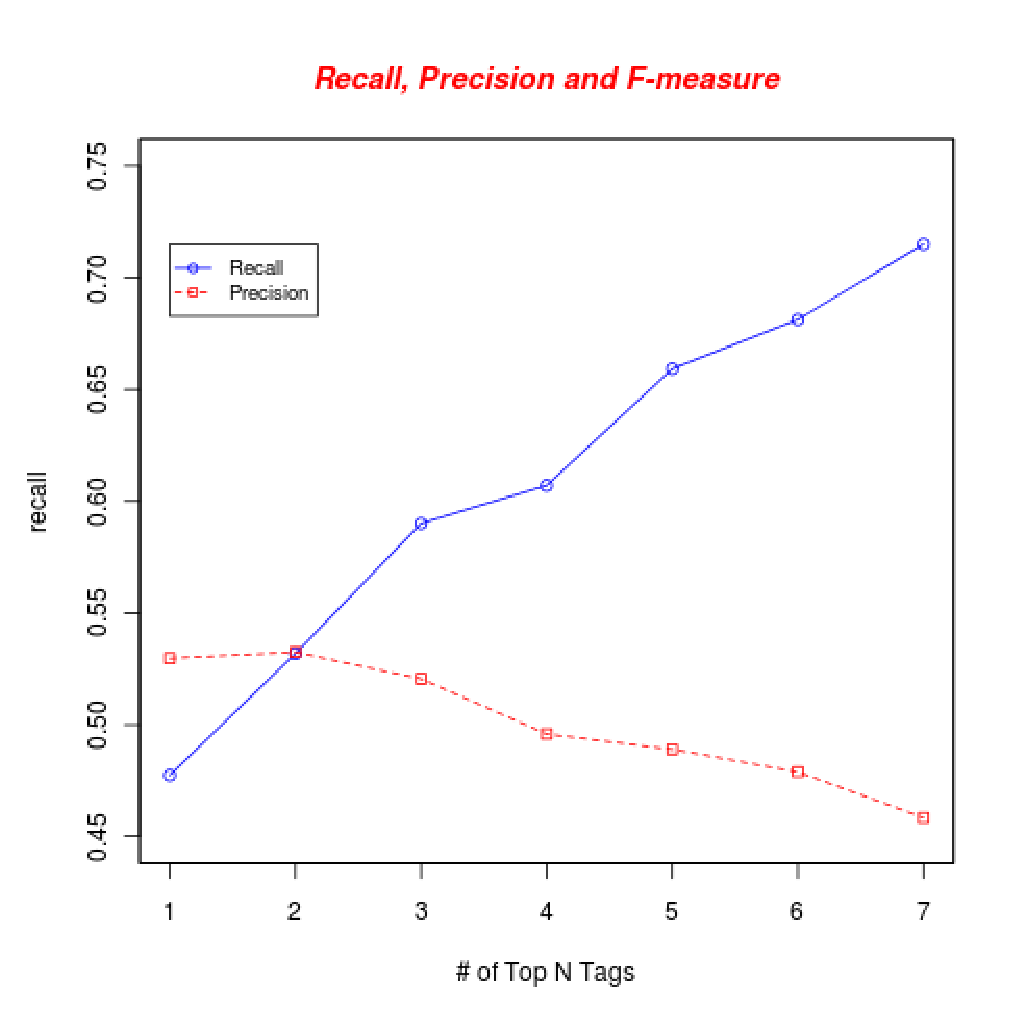
\includegraphics[scale=0.42]{naives.eps}
\caption{Tag Prediction By Naive Bayes}
\label{fig:naive}
\end{figure}

\subsubsection{Logistic Regression}
Under Construction

\subsubsection{Neural Networks}
Under Construction

\subsection{Comparison and Conclusion}
Under Construction. This part depends on the experimental results of all the three models.


\section{Reference}

% \small{
% [1] Alexander, J.A. \& Mozer, M.C. (1995) Template-based algorithms
% for connectionist rule extraction. In G. Tesauro, D. S. Touretzky
% and T.K. Leen (eds.), {\it Advances in Neural Information Processing
% Systems 7}, pp. 609-616. Cambridge, MA: MIT Press.
% 
% [2] Bower, J.M. \& Beeman, D. (1995) {\it The Book of GENESIS: Exploring
% Realistic Neural Models with the GEneral NEural SImulation System.}
% New York: TELOS/Springer-Verlag.
% 
% [3] Hasselmo, M.E., Schnell, E. \& Barkai, E. (1995) Dynamics of learning
% and recall at excitatory recurrent synapses and cholinergic modulation
% in rat hippocampal region CA3. {\it Journal of Neuroscience}
% {\bf 15}(7):5249-5262.
% }
% 
\end{document}
